\documentclass[12pt,a4paper]{article}
\usepackage[utf8]{inputenc}
\usepackage{amsmath}
\usepackage{amsfonts}
\usepackage{courier}
\usepackage{amssymb}
\usepackage{float}
\usepackage{graphicx}
\usepackage[left=1in,right=1in,top=1in,bottom=1in]{geometry}
\setlength\parindent{0pt}
\begin{document}
\title{MLND SmartCab Project Report}
\author{Juanyan Li}
\date{\today}
\maketitle

\section{Implement a Basic Driving Agent
}
The cabs are all moving in random directions, including not taking no action. However, they are still restricted by the enforced traffic rules (no forward and left turn on red light). In this fashion, althoug not likely, the primary agent (red cab) is still possible to reach the destination by chance (red spot, see Fig 1). 

\begin{figure}[H]
\caption{Reaching Destination}
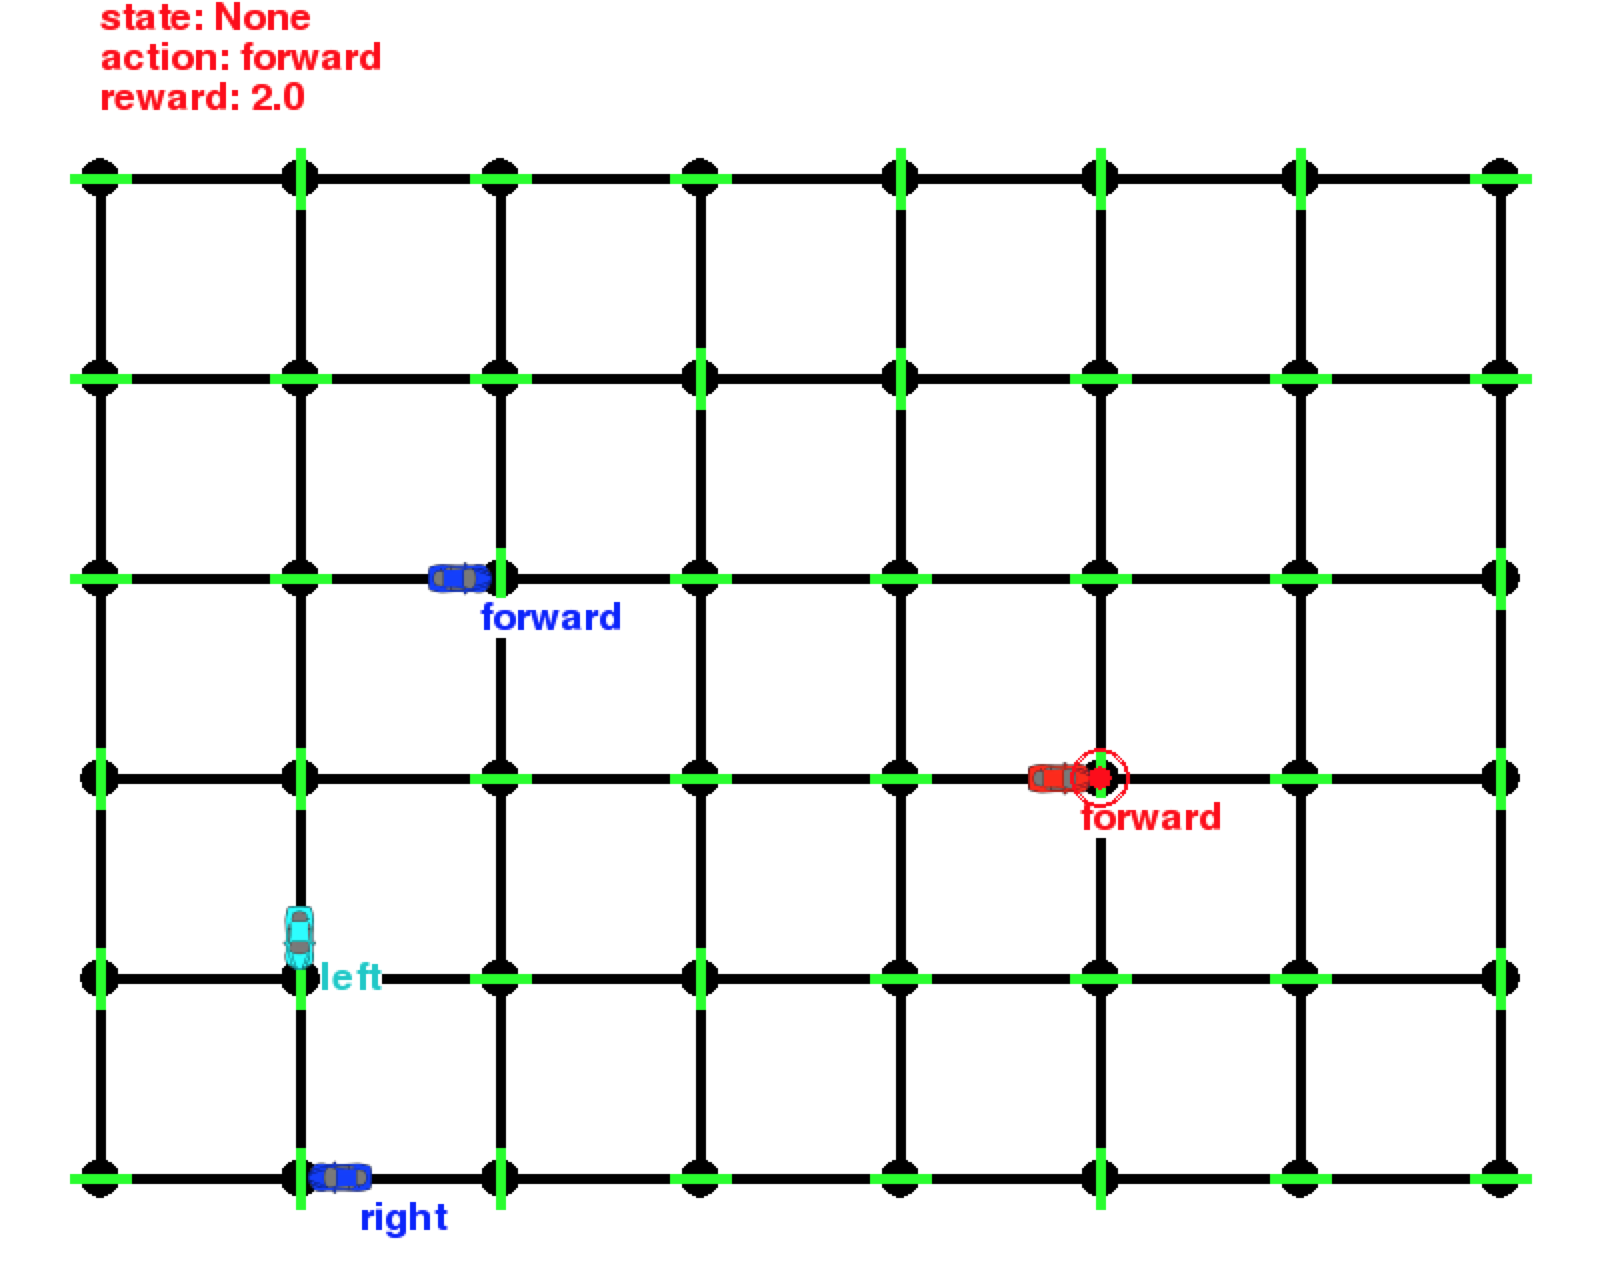
\includegraphics[width=12cm]{fig1.png}
\centering
\end{figure}

One interesting thing that I notice is the reward mechanism. There are 4 cases in total:

\begin{enumerate}
\item[(i)]
\textbf{Action is \texttt{None}}

Agent receives no reward when no action is taken at current time step (see Fig 2).
\begin{figure}[H]
\caption{No Action}
\includegraphics[width=12cm]{fig2.png}
\centering
\end{figure}

\item[(ii)]
\textbf{Action is prohibited by traffic rule}

Agent receives -1.0 reward when proposed action violated the traffic rule at current time step (see Fig 3).
\begin{figure}[H]
\caption{Violating Traffic Rules}
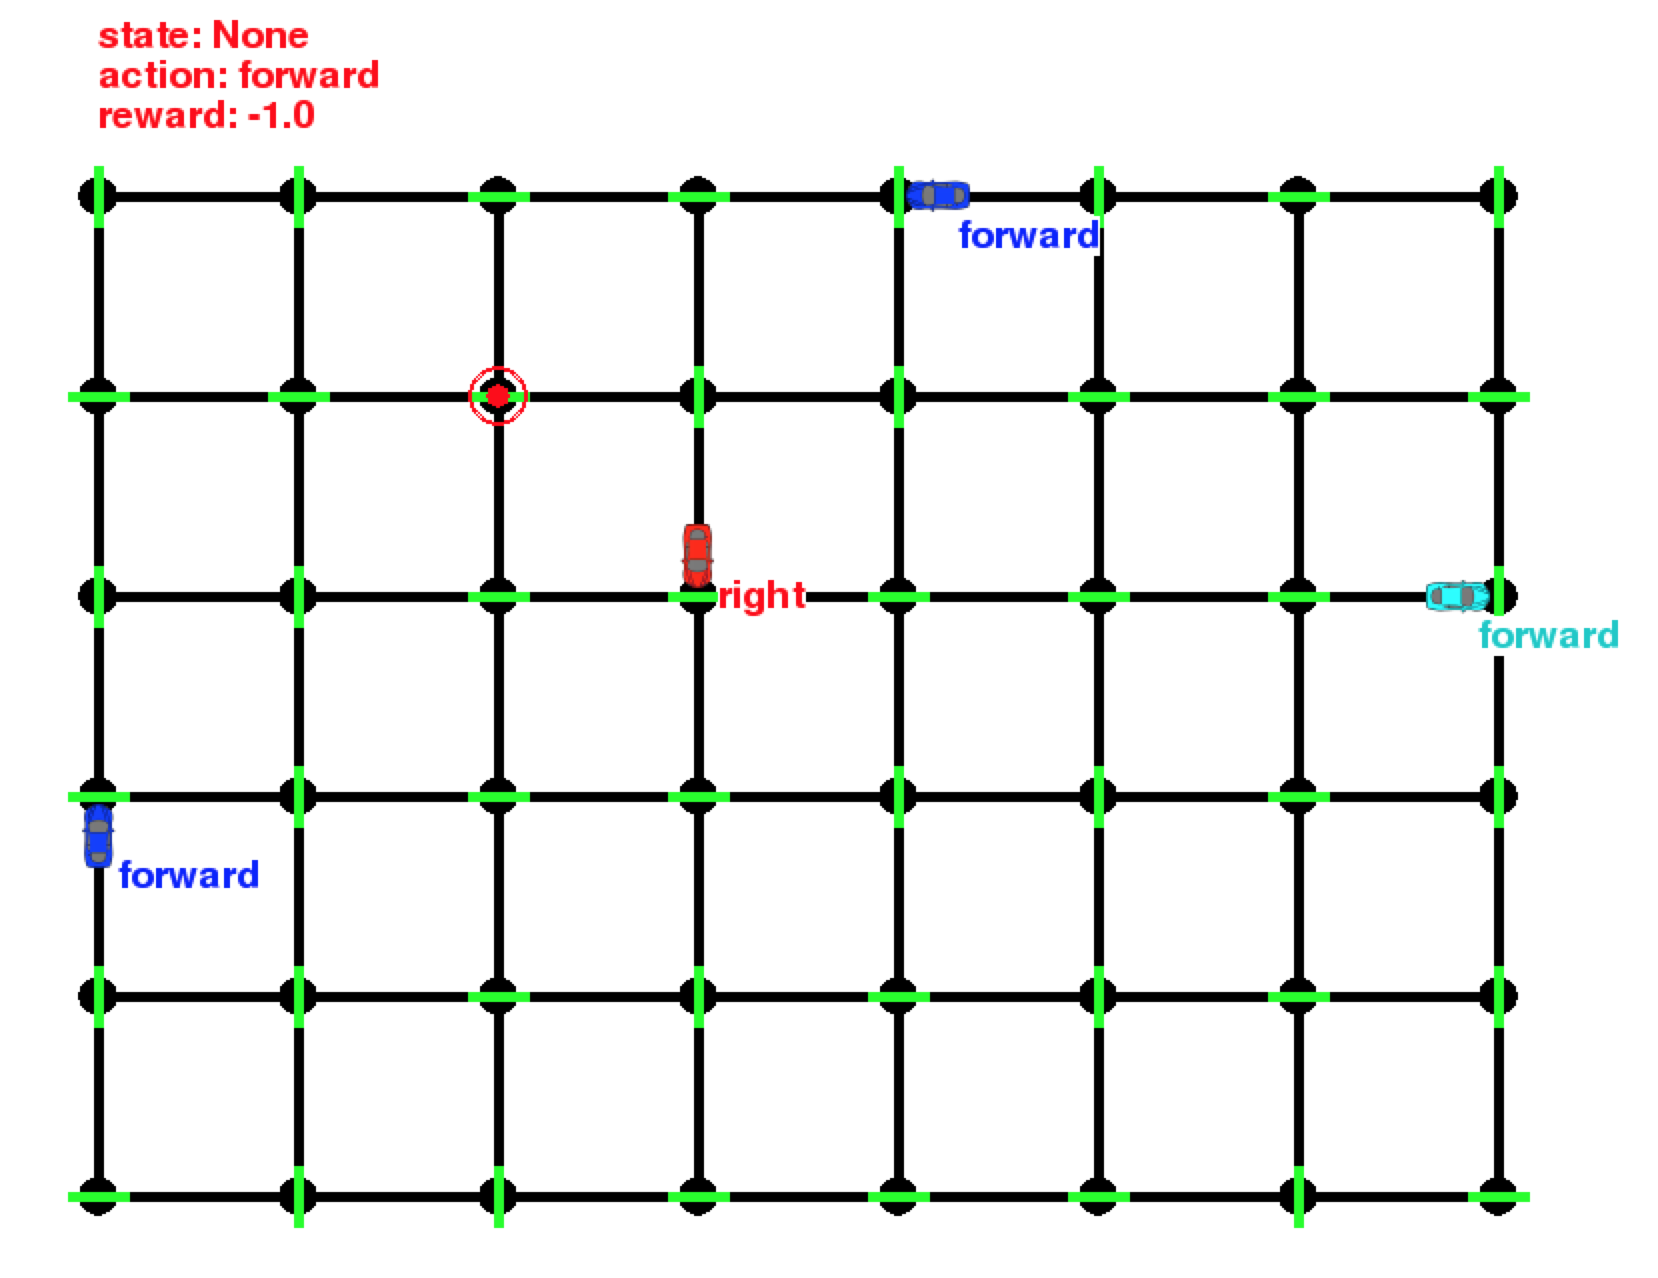
\includegraphics[width=12cm]{fig3.png}
\centering
\end{figure}

\item[(iii)]
\textbf{Action is moving away from destination}

Agent receives -0.5 reward when proposed action is heading away from destination (see Fig 4).
\begin{figure}[H]
\caption{Heading Towards Wrong Direction}
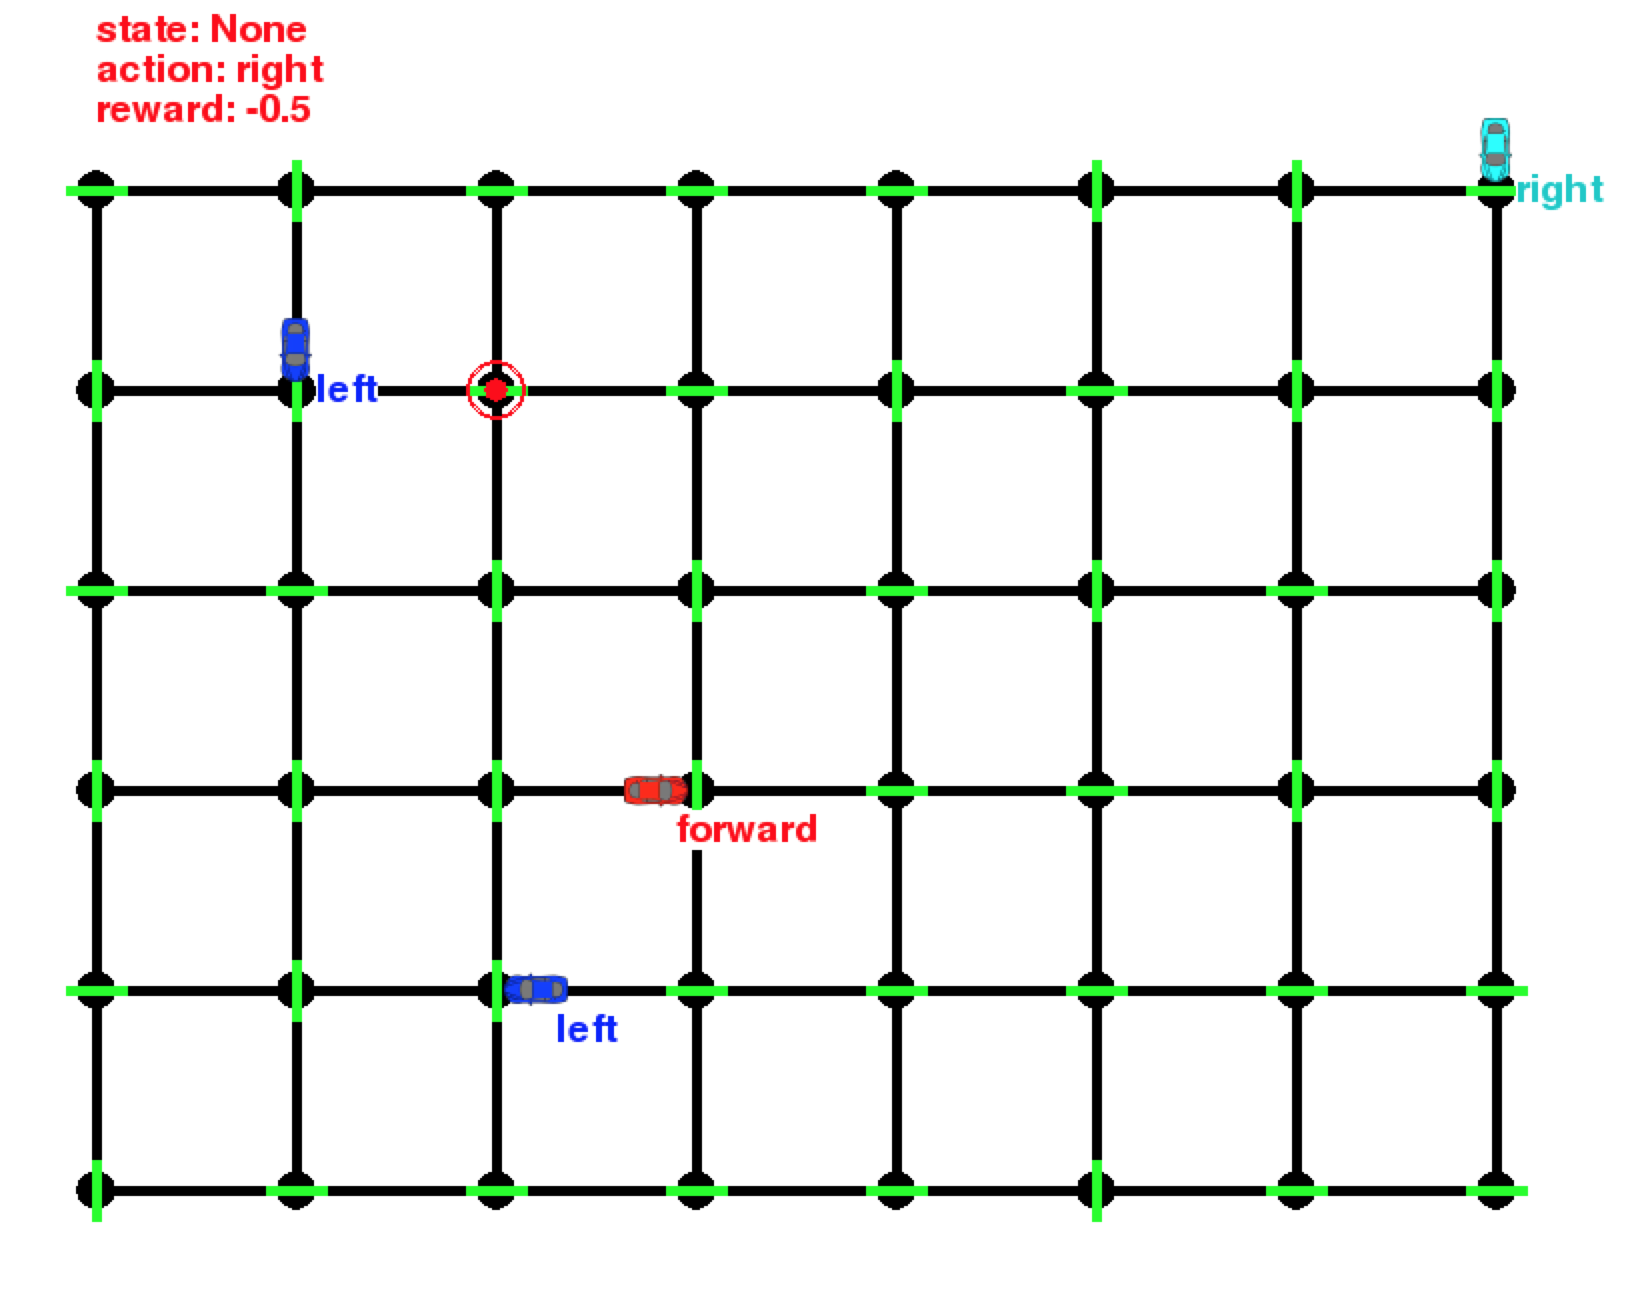
\includegraphics[width=12cm]{fig4.png}
\centering
\end{figure}

\item[(iv)]
\textbf{Action is moving towards destination}

Agent receives 2.0 reward when proposed action is heading towards destination (see Fig 5).
\begin{figure}[H]
\caption{Heading Towards Right Direction}
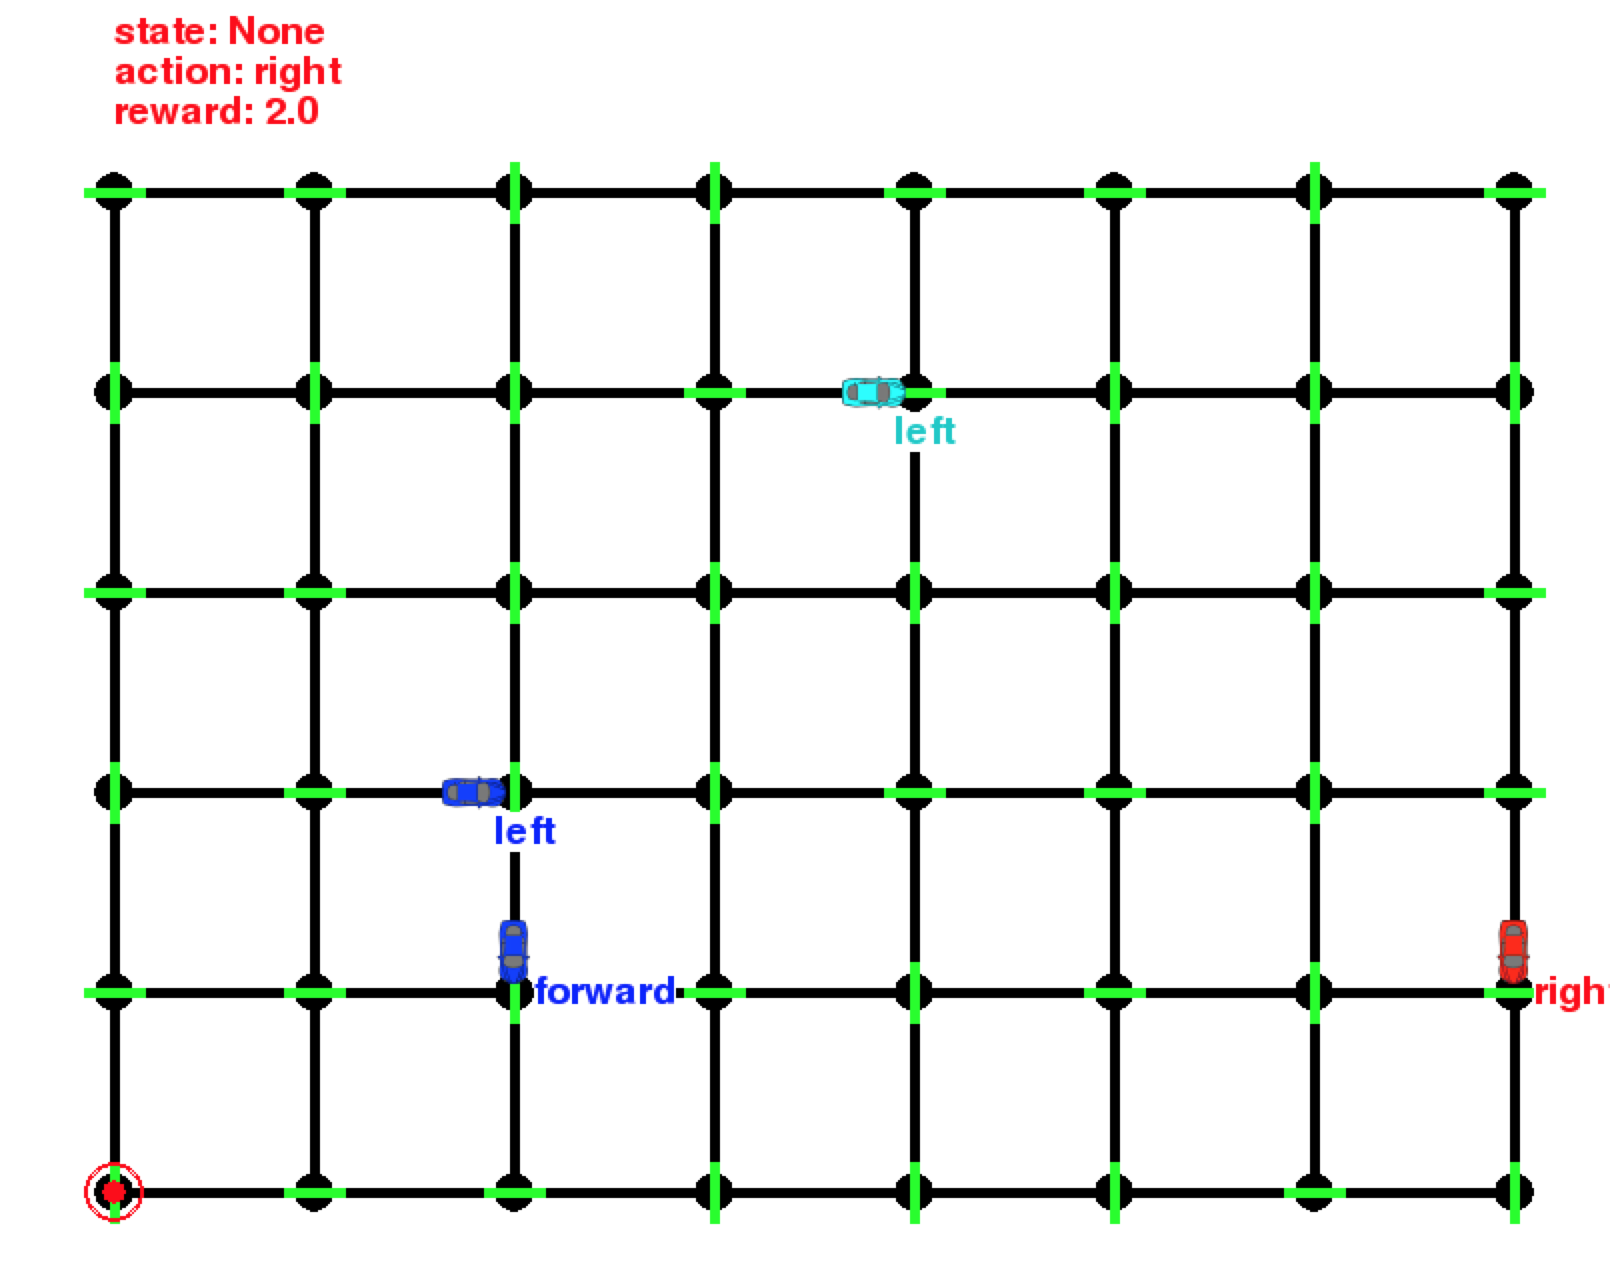
\includegraphics[width=12cm]{fig5.png}
\centering
\end{figure}

\end{enumerate}



\end{document}